\section{Theory}

	\subsection{Stuart-Landau-Oscillator}
	The Stuart-Landau oscillator is a dynamical system often used to model basic class 1 lasers. It can be written either as a single complex differential equation (\ref{eq:stuartlandauequation}) or a set of two equations written in polar coordinates (\ref{eq:stuartlandauequation_polar}). From the equation in polar coordinates easy to see that the equation has rotational symmetry as the radial differential equation does not change with the dynamical variable $\phi$.
	
	\begin{equation}	
		\dot{z} = (\lambda +  i \omega + \gamma |z|^2 ) \; z
		\label{eq:stuartlandauequation}		
	\end{equation}
	
	\begin{equation}
		\begin{split}
		\dot{r} & = \lambda r + \operatorname{Re} (\gamma) \; r^{3} \\
		\dot{\phi} &= i \omega + \operatorname{Im}(\gamma) \; r^{2} 
		\end{split}
		\label{eq:stuartlandauequation_polar}
	\end{equation}

	For the radial dynamical variable the Stuart-Landau oscillator has two fixed points where the derivative $\dot{r}$ vanishes $r = 0$ and $r = \sqrt{-\lambda /\operatorname{Re}(\gamma)}$ whose stability depends on $\lambda$ and $\operatorname{Re}(\gamma)$. For $\operatorname{Re}(\gamma) < 0 $ (supercritical case).
	

	\begin{figure}
		\centering
		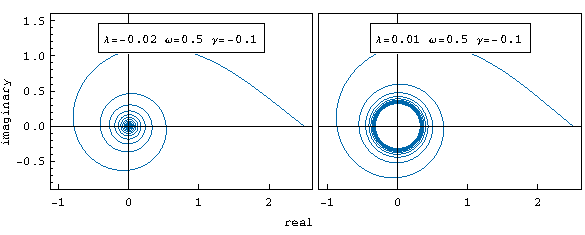
\includegraphics[width=0.99\linewidth]{pics/stuart_landau_complex_Focus_LC}
		\caption{$2$ very basic scenarios of the Stuart-Landau oscillator: Decay towards a single fixed point (left) or towards a limit cycle (right).}
		\label{fig:stuart_spiral}
		%nicht mehr
		%stuart_landau_basic.nb
	\end{figure}



The limit cycle (LC) which is shown in fig \ref{fig:stuart_spiral} is depending on the ratio or $\lambda$ and $Re \left[\gamma \right]$.





As can be seen in (eq. \ref{eq:stuartlandauequation}), the equation has a linear and a nonlinear term regarding the absolute value of $z$.

\subsection{Networks}

Vertices blabla \
Edges blabla. \

	\subsubsection{circulant Matrix}
    A circulant matrix has the same entries its row vectors, but with its entries rotated one element to the right relative to the previous row.
    
\subsection{virtual Nodes and multiplexing}
	here: papers for explanation!
	By multiplexing the input signal one can create virtual nodes in a network. The analogy to a real network can be best understood if the input signal is masked with a binary mask containing only values of either $0$ or $1$. 
	
	here add dependency of total linear memory on number of nodes and virtal nodes.

\begin{figure}
	\centering
	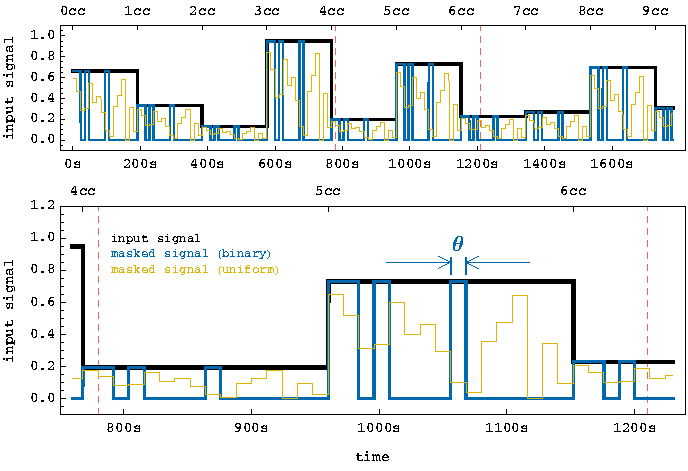
\includegraphics[width=0.99\linewidth]{pics/signal_mask_vis}
	\caption{A timeseries (black) with constant interpolation ("sample \& hold") between samples and the corresponding masked signal (blue). The mask length is counted in clockcycles (cc) and the time per virtual node is counted in $\theta$. Here $\theta = 12s$ and $1cc = 16 \theta = 272s $}
	\label{fig:signal_mask_vis}
	%feedInVis_stuartlandau.nb
\end{figure}

\subsection{Small world networks}
	The term small world network was introduced in \cite{WAT98a} and describes a predominately locally coupled network with few non-local edges. 
	

\subsection{Dynamics of rings of stuart landau oscillators}
	pony-states (von André)
	
	

% different stuart landau scenarios - hopf bifurcation